%-------------------------------------------------------------------------
% Class options include:
% print, %colors will be adjusted for printing 
% handout, %pauses will be disabled
% aspectratio=<parameter>, parameter = 1610,169,149,141,54,43(default),32
% e.g. \documentclass[aspectratio = 1610]{beamer}
%-------------------------------------------------------------------------

\documentclass{beamer}

\usetheme{ink} % theme ink


%-------------------------------------------------------------------------
% Loading packages
%-------------------------------------------------------------------------
\usetikzlibrary{shapes,arrows,decorations.pathmorphing,backgrounds,positioning,fit,petri}
\usepackage[ruled,vlined]{algorithm2e}


%-------------------------------------------------------------------------
% Title page
%-------------------------------------------------------------------------
\title{\LaTeX\ beamer Theme -- ink}
\subtitle{Manual}
\author{Xian Qiu}
\email{x.qiu@example.com}
%if using linebreak "\\", then also put a "\\" at text end 
\institute{Institution - 1st line \\ Institution - 2nd line \\}
%\inframeauthor{X.Qiu}
%\inframeinstitute{Institution Name}
\date{\today}

%-------------------------------------------------------------------------
% Begin
%-------------------------------------------------------------------------
\begin{document}

\maketitle


\begin{frame}[fragile]
	\frametitle{Using Theme -- ink}
	\begin{enumerate}
		\item put the following into the same folder with your \verb|tex| file
		\begin{itemize}
			\item folder: \verb|ink|
			\item file: \verb|beamerthemeink.sty|
		\end{itemize}
		\item use theme \verb|ink|
		\scriptsize
		\begin{verbatim}
		    \documentclass[10pt]{beamer}
		    \usetheme{ink}
		    \begin{document}
		        ...
		    \end{document}		    
		\end{verbatim}
	\end{enumerate}
	 
\end{frame}

\begin{frame}[fragile]
	\frametitle{Options}
	Class options include:
	\begin{itemize}
		\item \verb|print|: colors will be adjusted for printing
		\item \verb|handout|: pauses will be disabled
		\item \verb|aspectratio=<parameter>|: page size\\
		parameter = 1610,169,149,141,54,43(default),32
	\end{itemize}
	
	\scriptsize
	\begin{verbatim}
	    \documentclass[handout,print,aspectratio=1610]{beamer}
	        ...
	    \begin{document}
	        ...
	    \end{document}
	\end{verbatim}
\end{frame}

\begin{frame}[fragile]
	\frametitle{Title Page}
	\scriptsize
	\begin{verbatim}
	    \title{title of your presentation}
	    
	    \subtitle{subtitle}
	    
	    \author{Xian Qiu}
	    
	    \email{x.qiu@example.com}
	    
	    %if using "\\", then end text with "\\" 
	    \institute{Institution - 1st line \\ Institution - 2nd line \\}
	    
	    \date{\today} 
	    
	    %information shown at the bottom of slides
	    \inframeauthor{X. Qiu}
	    \inframeinstitute{Institution Name}
	\end{verbatim}
	
\end{frame}

\begin{frame}[fragile]
	\frametitle{Frames} 
	\scriptsize
	\begin{minipage}{0.6\textwidth}
		\begin{verbatim}
		\begin{chapterframe} 
		    \frametitle{Outline} ...
		\end{chapterframe}
		
		
		\begin{frame } % this slide
		    \frametitle{Title of the Frame}
		\end{frame }
		
		
		\begin{thanksframe}
		    \frametitle{Thank you!}
		\end{thanksframe}
		\end{verbatim}
	\end{minipage}\begin{minipage}{0.3\textwidth}
	\begin{tikzpicture}
	    \node[draw] (chpfm) {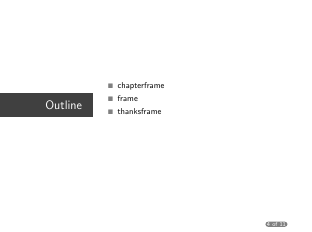
\includegraphics[scale=0.35]{gfx/chpfm.png}};
	    \node[draw] (thkfm) [below = of chpfm] {
\includegraphics[scale=0.35]{gfx/thkfm}};
	\end{tikzpicture}
\end{minipage}
	
\end{frame}


\begin{frame}[fragile]
	\frametitle{Theorems}
	
	\begin{theorem}
		If $Q/\sigma^2 \sim \chi^2(r)$ and $Q_i/\sigma^2 \sim \chi^2(r_i)$ for $i=1,\ldots,k-1$, then
		\begin{enumerate}
			\item $Q_1,\ldots,Q_k$ are independent;
			\item $Q_k/\sigma^2 \sim \chi^2(r_k)$, where $r_k = r - \sum_{i=1}^{n}r_i$.
		\end{enumerate}
	\end{theorem}
	\begin{proof}
		content...
	\end{proof}
	
	\scriptsize
	\begin{verbatim}
	\begin{theorem}
	    ...
	\end{theorem}
	\begin{proof}
	    ...
	\end{proof}
	\end{verbatim}
\end{frame}

\begin{frame}[fragile]
	\frametitle{Blocks}
	\begin{block}{Block Title}
		content...
	\end{block}
	
	\scriptsize
	\begin{verbatim}
	\begin{block}{Block Title}
	    content...
	\end{block}
	\end{verbatim}
\end{frame}

\begin{frame}[fragile]
	\frametitle{Stickers}
    \blacksticker{(5,3)}{this is a black sticker}
    \yellowsticker{(-4,1)}{this is a yellow sticker}
    \redsticker{(4,7)}{this is a red sticker}
    \orangesticker{(7,5)}{this is an orange sticker}
    \bluesticker{(1,6)}{this is a blue sticker}
    \greensticker{(3,4)}{this is a green sticker}
    
    \scriptsize
    \begin{verbatim}
    
    
    
        \blacksticker{(5,3)}{this is a black sticker}
        
        
        \greensticker{(3,4)}{this is a green sticker}
        
        
        \orangesticker{(7,5)}{this is an orange sticker}
        
        
        \bluesticker{(1,6)}{this is a blue sticker}
        
        
        \redsticker{(4,7)}{this is a red sticker} 
        
          
    \end{verbatim}
\end{frame}

\begin{frame}[fragile]
	\frametitle{Useful Commands}
	\scriptsize
	\begin{itemize}
		\item \verb|\tgray|: \tgray{hint text}
		\item \verb|\tred|: \tred{emphasize text red }
		\item \verb|\tblue|: \tblue{emphasize text blue}
		\item \verb|\set|: $\set{1,2,\ldots,n}$
		\item \verb|\abs|: $\abs{\text{absolute value}}$ 
    \end{itemize}

\end{frame}

\end{document}
